% !TEX encoding = UTF-8 Unicode

%
% Exemple de rapport
% par Pierre Tremblay, Universite Laval
% modifié par Christian Gagne, Universite Laval
% modifié par Francis Valois, Université Laval
% 31/01/2011 - version 1.4
%

%
% Modele d'organisation d'un projet LaTeX 
% rapport/      dossier racine et fichier principal
% rapport/fig   fichiers des figures
% rapport/tex   autres fichiers .tex
%

% ** Preambule **
%
% Ajouter les options au besoin :
%    - "ULlof" pour inclure la liste des figures, requis si "\begin{figure}" utilise
%    - "ULlot" pour inclure la liste des tableaux, requis si "\begin{table}" utilise
%
\documentclass[12pt,ULlof,ULlot]{ULrapport}

% Chargement des packages supplementaires (si absent de la classe)
\usepackage[utf8]{inputenc}
\usepackage[T1]{fontenc}
\usepackage[autolanguage]{numprint}
\usepackage{icomma}
\usepackage{subfigure}
\usepackage{graphicx}
\usepackage[absolute]{textpos}
\usepackage[final]{pdfpages}
\def\dbar{{\mathchar'26\mkern-12mu d}} 
%\usepackage[options]{nom_du_package}

% Definition d'une commande pour presenter des cellules multilignes dans un tableau
\newcommand{\cellulemultiligne}[1]{\begin{tabular}{@{}c@{}}#1\end{tabular}}


% Definition de colonnes en mode paragraphe avec alignement ajustable
% Cette definition requiert le chargement du package "array"
%    - alignement horizontal, parametre #1 : - \raggedright (aligne a gauche)
%                                            - \centering (centre)
%                                            - \raggedleft (aligne a droite)
%    - alignement vertical, parametre #2 : - p (aligne en haut)
%                                          - m (centre)
%                                          - b (aligne en bas)
%    - largeur, parametre #3 : longueur
\newcolumntype{Z}[3]{>{#1\hspace{0pt}\arraybackslash}#2{#3}}

% Definitions des parametres de la page titre
\TitreProjet{Livrable 1 - Robot Kinocto}                         % Titre du projet
\TitreRapport{Machines Électriques}       % Titre du rapport
\Destinataire{M. Dominique Grenier, M. Luc Lamontagne et M. Abdelhakim Bendada}         % Nom(s) du destinataire
\TableauMembres{%                                     % Tableau des membres de l'equipe
   XXX\,XXX\,XXX  & Émile Arsenault \\\hline 
   908\,190\,985  & Philippe Bourdages \\\hline
   910\,098\,468  & Pierre-Luc Buhler \\\hline    
   XXX\,XXX\,XXX & Diane Fournier \\\hline
   908\,159\,170  & Imane Mouhtij \\\hline
   XXX\,XXX\,XXX  & Olivier Sylvain \\\hline
   XXX\,XXX\,XXX  & Daniel Thibodeau \\\hline
   XXX\,XXX\,XXX  & Francis Valois \\\hline
}
\DateRemise{11 février 2012}                           % Date de remis


% Corps du document

\begin{document}

%   Chapitres
%!TEX root = ../rapport.tex
%!TEX encoding = UTF-8 Unicode

% Chapitres "Introduction"

% modifié par Francis Valois, Université Laval
% 31/01/2011 - version 1.0 - Création du document

\chapter{Introduction}
\label{s:introduction}

%!TEX root = ../rapport.tex
%!TEX encoding = UTF-8 Unicode

% Chapitres "Introduction"

% modifié par Francis Valois, Université Laval
% 31/01/2011 - version 1.0 - Création du document

\chapter{Diagramme de contexte}
\label{s:contexte}
\begin{figure}[htb]
\centering
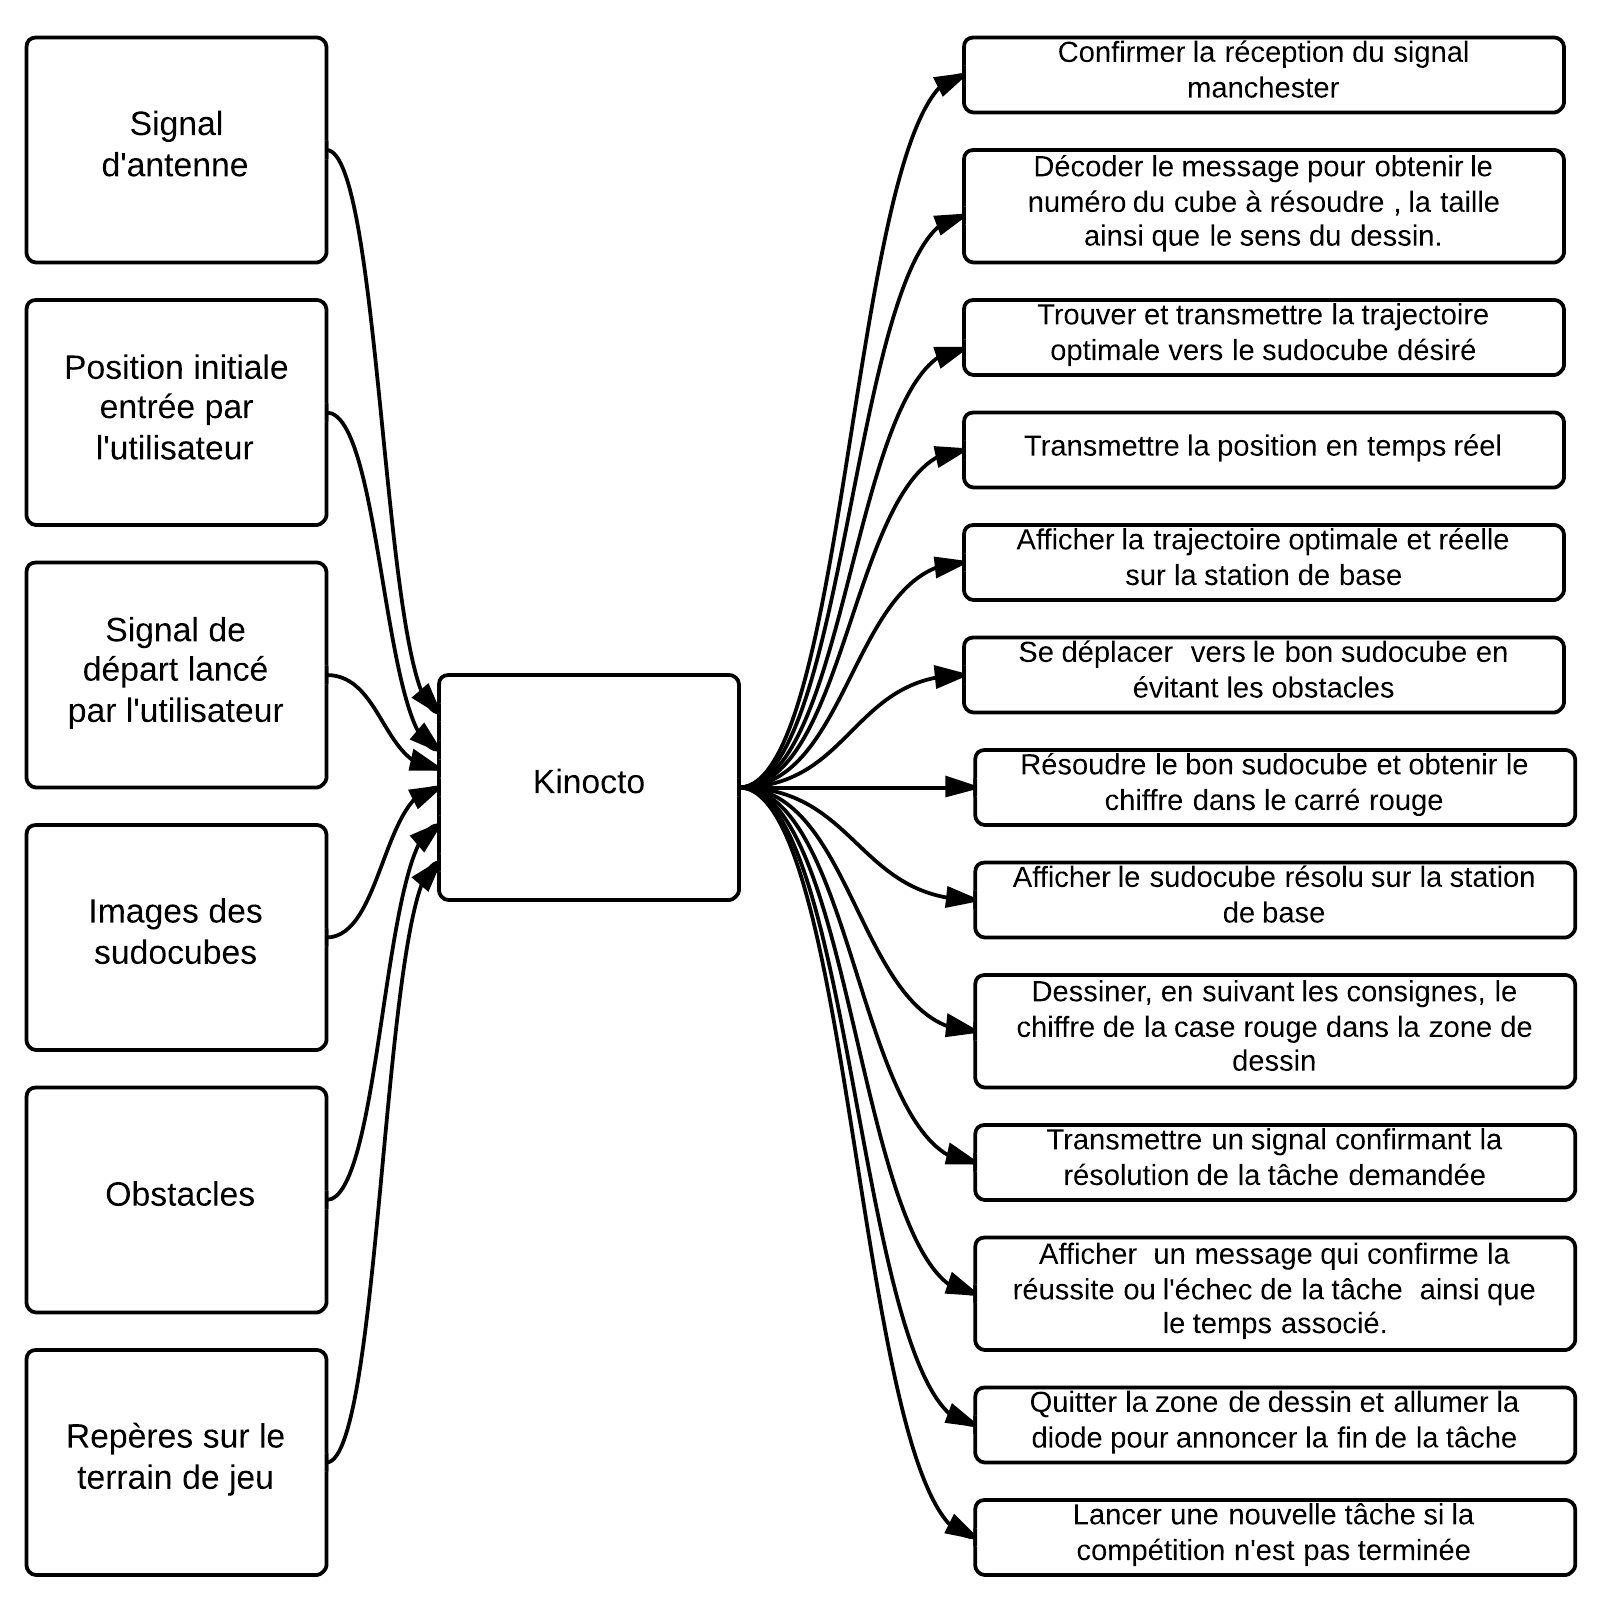
\includegraphics[scale=0.38]{fig/DiagrammeDeContexteDesign3.png}
\end{figure}

%!TEX root = ../rapport.tex
%!TEX encoding = UTF-8 Unicode

% Chapitres "Introduction"

% modifié par Francis Valois, Université Laval
% 31/01/2011 - version 1.0 - Création du document
\chapter{Description des propriétés fonctionnelles}
\label{s:fonctionnelles}
Pour simplifier la lecture du tableau de la description des propriétés fonctionnelles, celui-ci a été séparé en trois pages selon trois différentes sections: vision et traitement numérique (présenté dans le tableau \ref{tab:dpf1}), communication et déplacement (présenté dans le tableau \ref{tab:dpf2}) ainsi qu'alimentation et affichage (présenté dans le tableau \ref{tab:dpf3}). 

\newlength{\hcolw}
\setlength{\hcolw}{\textwidth}
\eject \pdfpagewidth=15.7in \pdfpageheight=10in
\textwidth=13.7in

\begin{table}[!ht]
\centering
	\begin{minipage}[c]{13.8in}
	\caption{Description des propriétés fonctionnelles: section "Vision et Traitement Numérique"} 
	\label{tab:dpf1}
	\small
	\scalebox{0.8}{
	\tabcolsep=0.11cm
	\begin{tabular}{|Z{\raggedright}{m}{6.5cm}||Z{\centering}{m}{1.5cm}|Z{\centering}{m}{1.5cm}|Z{\centering}{m}{1.5cm}|Z{\centering}{m}{1.5cm}|Z{\centering}{m}{1.5cm}|Z{\centering}{m}{1.5cm}|Z{\centering}{m}{2cm}|Z{\centering}{m}{1.5cm}|Z{\centering}{m}{1.5cm}|Z{\centering}{m}{1.5cm}|Z{\centering}{m}{1.5cm}|Z{\centering}{m}{2.3cm}|Z{\centering}{m}{1.5cm}|Z{\centering}{m}{2cm}|Z{\centering}{m}{2cm}|Z{\centering}{m}{3cm}|Z{\centering}{m}{2cm}|Z{\centering}{m}{2cm}|} 
		
		\cline{2-19}
		\multicolumn{1}{c|}{} 																						& \multicolumn{18}{c|}{\textbf{Fonctionnalités}} \\ \cline{2-19}
		\multicolumn{1}{c|}{} 																						& \multicolumn{10}{c|}{Vision numérique} 																		& \multicolumn{8}{c|}{Traitement numérique}																																											\\ \cline{2-19}
		\multicolumn{1}{c|}{} 																						& \multicolumn{3}{Z{\centering}{m}{5cm}|}{Détecter obstacles} 	& \multicolumn{4}{Z{\centering}{m}{7cm}|}{Localiser le robot} 		& \multicolumn{3}{Z{\centering}{m}{5cm}|}{Lire le cube} 			&  \multicolumn{2}{Z{\centering}{m}{4cm}|}{Calculer la trajectoire optimale}	& \multicolumn{2}{Z{\centering}{m}{4cm}|}{Contrôler le robot pour le dessin} 	& Décoder le signal d'antenne 	& Choisir le cube selon le signal d'antenne & \multicolumn{2}{Z{\centering}{m}{4cm}|}{Résoudre le sudocube}  \\ \hline
		\centering\textbf{Exigences du client}																		& Temps de calcul (s) & Précision en X (cm) & Précision en Z (cm) & Temps de calcul (s) & Précision en X (cm) & Précision en Z (cm) & Précision angulaire ($^o$)  & Temps de calcul (s) 	& Distance min (m) & Distance max(m) & Temps de calcul (s) & Nombre de déplacement maximum & Temps de calcul (s) 	& Précision (cm) 									& 	Nombre de périodes nécessaires	& 											& Temps de calcul (s) 	& Chiffres initiaux minimum\\ \hline  \hline
		Être autonome pendant un minimum de 10 minutes 																& 2 & 4 & 4 & 2 & 5 & 5 & 4 & 5 & 3 & 1 & 2 & 2 & 3 & 3 & 2 & 4 & 2 & 1 \\ \hline
		Se déplacer selon la trajectoire optimale																	& 3 & 5 & 5 & 3 & 5 & 5 & 5 &  &  &  & 5 & 5 &  &  & 3 & 3 &  &  \\ \hline
		Effectuer une séquence complète en moins de 10 minutes 														& 5 & 3 & 3 & 5 & 3 & 3 & 3 & 5 & 3 & 1 & 5 & 3 & 5 &  &  & 3 & 3 & 2 \\ \hline
		Alimenter le Mac mini avec une tension de 22V à 30V et ondulation de tension inférieure à 200 mV 			&  &  &  &  &  &  &  &  &  &  &  &  &  &  &  &  &  &  \\ \hline
		Résoudre sudocube 																							&  &  &  &  &  &  &  & 5 & 3 & 1 &  &  &  &  &  &  & 5 & 5 \\ \hline
		Dessiner le chiffre selon le signal d'antenne dans une zone prédéfinie (jaune) avec une précision de ± 1cm 	&  &  &  &  &  &  &  &  &  &  &  &  &  & 5 &  &  &  &  \\ \hline
		Éviter les obstacles ainsi que les murs de la table															& 3 & 5 & 5 & 3 & 5 & 5 & 5 &  &  &  & 3 & 5 &  &  &  &  &  &  \\ \hline
		Décoder le signal d'antenne																					&  &  &  &  &  &  &  &  &  &  &  &  &  &  & 5 &  &  &  \\ \hline
		Analyser le bon cube selon le signal d'antenne 																&  &  &  &  &  &  &  &  &  &  &  &  &  &  &  & 5 & 5 & 1 \\ \hline
		Utiliser la communication sans fil 																			&  &  &  &  &  &  &  &  &  &  &  &  &  &  &  &  &  &  \\ \hline
		Concevoir un système de préhension pour le crayon 															&  &  &  &  &  &  &  &  &  &  &  &  &  & 3 &  &  &  &  \\ \hline 
		Afficher position réelle																					&  &  &  & 3 & 5 & 5 & 5 &  &  &  &  &  &  &  &  &  &  &  \\ \hline
		Afficher la trajectoire optimale 																			& 3 & 5 & 5 & 3 & 5 & 5 & 5 &  &  &  & 3 & 5 &  &  & 3 & 5 &  &  \\ \hline
		Afficher le cube résolu et le chiffre de la case rouge sur la base 											&  &  &  &  &  &  &  & 5 & 2 & 2 &  &  &  &  &  &  & 5 & 5 \\ \hline
		Allumer une DEL lorsque tâche terminée 																		&  &  &  &  &  &  &  &  &  &  &  &  &  &  &  &  &  &  \\ \hline 
		Afficher message de fin 																					&  &  &  &  &  &  &  &  &  &  &  &  &  &  &  &  &  &  \\ \hline
		Afficher message de départ 																					&  &  &  &  &  &  &  &  &  &  &  &  &  &  &  &  &  &  \\ \hline
		Afficher trajectoire réelle avec un délai maximum de 15s 													&  &  &  & 3 & 5 & 5 & 5 &  &  &  &  &  &  &  &  &  &  &  \\ \hline
		Afficher les informations sur le robot 																		&  &  &  &  &  &  &  &  &  &  &  &  &  &  &  &  &  &  \\ \hline
		Le robot doit se retirer de la zone de dessin une fois celui-ci terminée									&  &  &  &  &  &  &  &  &  &  &  &  &  &  &  &  &  &  \\ \hline 
		Respecter un budget de 250\$ 																				&  &  &  &  &  &  &  &  &  &  &  &  & 3 & 5 & 3 &  &  &  \\ \hline 
		Respecter l'échéancier																						& 3 & 5 & 5 & 3 & 5 & 5 & 3 & 5 & 1 & 1 & 3 & 3 & 1 & 5 & 3 & 3 & 5 & 3 \\ \hline
	\end{tabular}}
	\end{minipage}
\end{table}

\newpage
\eject \pdfpagewidth=15.7in 

\begin{table}[!ht]
\makebox[\textwidth][c]{
\begin{minipage}[c]{12.5in}
	\caption{Description des propriétés fonctionnelles: section "Communication et Déplacement"} 
	\label{tab:dpf2}
	\small
	\scalebox{0.8}{
	\tabcolsep=0.11cm
	\begin{tabular}{|Z{\raggedright}{m}{6.5cm}||Z{\centering}{m}{2cm}|Z{\centering}{m}{2cm}|Z{\centering}{m}{2cm}|Z{\centering}{m}{4cm}|Z{\centering}{m}{1.5cm}|Z{\centering}{m}{1.5cm}|Z{\centering}{m}{4cm}|Z{\centering}{m}{4cm}|Z{\centering}{m}{1.5cm}|Z{\centering}{m}{1.5cm}|Z{\centering}{m}{2.5cm}|Z{\centering}{m}{2cm}|Z{\centering}{m}{1.5cm}|} 
		
		\cline{2-14}
		\multicolumn{1}{c|}{} 																						& \multicolumn{13}{c|}{\textbf{Fonctionnalités}} \\ \cline{2-14}
		\multicolumn{1}{c|}{} 																						& \multicolumn{11}{c|}{Communication} & \multicolumn{2}{c|}{Déplacement}\\ \cline{2-14}
		\multicolumn{1}{c|}{} 																						& \multicolumn{1}{Z{\centering}{m}{2cm}|}{Recevoir le signal d'antenne} & \multicolumn{2}{Z{\centering}{m}{4cm}|}{Communiquer entre le robot et la station de base}  & Communiquer entre le Mac mini et le microcontrôleur & \multicolumn{2}{Z{\centering}{m}{3cm}|}{Commander les moteurs} & Transmettre les images de la Kinect vers le Mac & Transmettre les images de la caméra vers le Mac & \multicolumn{2}{Z{\centering}{m}{3cm}|}{Contrôler la position de la caméra}  & Commander le préhenseur du crayon & \multicolumn{2}{Z{\centering}{m}{3.5cm}|}{Se déplacer sans toucher aux obstacles} \\ \hline
		\centering\textbf{Exigences du client}																		&  & Vitesse (Mo/s) & Latence (ms) &Vitesse (bits/s) &  Précision (cm) &  Temps de réponse (s) & Taux de transfert (images/s) & Taux de transfert(images/s) & Temps de réponse (s) & Précision (degré) & Temps de réponse (s) & Résolution (Degrés) & Vitesse (m/s) \\ \hline  \hline
		Être autonome pendant un minimum de 10 minutes 																& 4     & 3     & 3     & 5     & 5     & 5     & 5     & 5     & 1     & 1     & 4     & 3     & 1 \\ \hline
    	Se déplacer selon la trajectoire optimale 																	& 3     &       &       & 3     & 5     & 5     & 5     & 2     &       &       &       & 5     & 5 \\ \hline
    	Effectuer une séquence complète en moins de 10 minutes 														& 5     &       &       & 3     & 4     & 3     & 5     &       &       &       &       & 5     & 5 \\ \hline
  		Alimenter le Mac mini avec une tension de 22V à 30V et ondulation de tension inférieure à 200 mV 			&       &       &       &       &       &       &       &       &       &       &       &       &  \\ \hline
    	Résoudre sudocube 																							&       &       &       &       &       &       &       & 3     & 1     & 1     &       &       &  \\ \hline
 		Dessiner le chiffre selon le signal d'antenne dans une zone prédéfinie (jaune) avec une précision de ± 1cm 	&       &       &       & 5     & 5     & 5     & 3     &       &       &       & 5     & 5     & 5 \\ \hline
    	Éviter les obstacles ainsi que les murs de la table 														&       &       &       & 5     & 3     & 3     & 5     & 4     &       &       &       & 5     &  \\ \hline
    	Décoder le signal d'antenne 																				&       &       &       & 2     &       &       &       &       &       &       &       &       &  \\ \hline
    	Analyser le bon cube selon le signal d'antenne 																& 5     &       &       &       &       &       &       &       &       &       &       &       &  \\ \hline
    	Utiliser la communication sans fil  																		&       & 5     & 5     &       &       &       & 5     &       &       &       &       &       &  \\ \hline
    	Concevoir un système de préhension pour le crayon  															&       &       &       &       &       &       &       &       &       &       & 5     &       &  \\ \hline
    	Afficher position réelle 																					&       & 5     & 5     & 5     &       &       & 5     &       &       &       &       &       &  \\ \hline
    	Afficher la trajectoire optimale 																			& 3     & 5     & 2     & 3     &       &       & 5     &       &       &       &       &       &  \\ \hline
    	Afficher le cube résolu et le chiffre de la case rouge sur la base 											&       & 5     & 2     &       &       &       &       & 3     &       &       &       &       &  \\ \hline
    	Allumer une DEL lorsque tâche terminée 																		&       &       &       & 5     &       &       &       &       &       &       &       &       &  \\ \hline
    	Afficher message de fin 																					&       & 5     & 1     &       &       &       &       &       &       &       &       &       &  \\ \hline
    	Afficher message de départ 																					&       & 5     & 1     &       &       &       &       &       &       &       &       &       &  \\ \hline
    	Afficher trajectoire réelle avec un délai maximum de 15s 													&       & 5     & 5     & 5     &       &       & 5     &       &       &       &       &       &  \\ \hline
    	Afficher les informations sur le robot 																		&       &       &       & 5     &       &       &       &       &       &       &       &       &  \\ \hline
    	Le robot doit se retirer de la zone de dessin une fois celui-ci terminé 									&       &       &       & 5     & 5     & 1     &       &       &       &       &       & 5     &  \\ \hline
    	Respecter un budget de 250\$ 																				& 3     &       &       & 1     & 5     & 1     &       &       &       &       & 2     &       &  \\ \hline 
    	Respecter l'échéancier 																						& 3     & 3     & 2     & 3     & 5     & 2     & 5     & 3     & 1     & 1     & 5     & 3     & 3 \\ \hline

	\end{tabular}}
	\end{minipage}}
\end{table}

\newpage
\eject \pdfpagewidth=15.7in 

\begin{table}[!ht]
\makebox[\textwidth][c]{
\begin{minipage}[c]{12.85in}
	\caption{Description des propriétés fonctionnelles: section "Alimentation et affichage"} 
	\label{tab:dpf3}
	\small
	\scalebox{0.8}{
	\tabcolsep=0.11cm
	\begin{tabular}{|Z{\raggedright}{m}{6.5cm}||Z{\centering}{m}{1.5cm}|Z{\centering}{m}{2cm}|Z{\centering}{m}{2.5cm}|Z{\centering}{m}{2cm}|Z{\centering}{m}{1.8cm}|Z{\centering}{m}{2.2cm}|Z{\centering}{m}{2cm}|Z{\centering}{m}{2cm}|Z{\centering}{m}{2cm}|Z{\centering}{m}{2cm}|Z{\centering}{m}{2.1cm}|Z{\centering}{m}{2cm}|Z{\centering}{m}{3cm}|Z{\centering}{m}{1.5cm}|Z{\centering}{m}{1.5cm}|} 
		
		\cline{2-16}
		\multicolumn{1}{c|}{} 																						& \multicolumn{15}{c|}{\textbf{Fonctionnalités}} \\ \cline{2-16}
		\multicolumn{1}{c|}{} 																						& \multicolumn{8}{c}{Alimentation} & \multicolumn{7}{|c|}{Affichage}\\ \cline{2-16}
		\multicolumn{1}{c|}{} 																						& \multicolumn{3}{Z{\centering}{m}{6.5cm}|}{Utiliser une pile rechargeable} & Alimenter les moteurs & \multicolumn{2}{Z{\centering}{m}{4.3cm}|}{Alimenter le Mac} & \multicolumn{2}{Z{\centering}{m}{4.5cm}|}{Alimenter les différents périphériques }& Afficher message d'initiation de la tâche & Afficher le cube résolu ainsi que la case rouse & Allumer la DEL lorsque tâche complétée & Afficher la trajectoire optimale & Afficher la position et trajectoire réelle & Afficher message de fin & Afficher sur le LCD\\ \hline
		\centering\textbf{Exigences du client}																		& Énergie (Wh) & Courant maximal (A) & Durée d'une charge (min) & Puissance (W) & Puissance (W) & Ondulation de tension (mV) & Puissance (W) & Ondulation de tension (mV) & Puissance (W) &  &  &  & Temps d'actualisation (s) &  &    \\ \hline  \hline
		Être autonome pendant un minimum de 10 minutes 																& 5     & 3     & 5     & 3     & 3     & 3     & 3     & 5     &       &       &       &       &       &       &  \\ \hline
    	Se déplacer selon la trajectoire optimale 																	& 5     & 3     & 1     & 5     & 5     & 5     & 3     & 3     &       &       &       &       &       &       &  \\ \hline
    	Effectuer une séquence complète en moins de 10 minutes 														& 5     & 3     & 2     & 5     & 5     & 5     & 5     & 5     &       &       &       &       &       &       &  \\ \hline
    	Alimenter le Mac mini avec une tension de 22V à 30V et ondulation de tension inférieure à 200 mV			& 5     & 5     & 3     &       & 5     & 5     & 3     & 3     &       &       &       &       &       &       &  \\ \hline
    	Résoudre sudo-cube 																							& 5     & 5     & 2     &       & 5     & 5     & 5     & 5     &       &       &       &       &       &       &  \\ \hline
    	Dessiner le chiffre selon le signal d'antenne dans une zone prédéfinie (jaune) avec une précision de ± 1cm 	& 3     & 3     & 1     & 3     & 3     & 3     & 3     & 3     &       &       &       &       &       &       &  \\ \hline
    	Éviter les obstacles ainsi que les murs de la table 														& 3     & 3     & 1     & 3     & 3     & 3     & 3     & 3     &       &       &       &       &       &       &  \\ \hline
	    Décoder le signal d'antenne 																				& 5     & 3     & 1     &       & 3     & 3     & 5     & 5     &       &       &       &       &       &       & 3 \\ \hline
	    Analyser le bon cube selon le signal d'antenne 																& 5     & 2     & 1     &       & 1     & 2     & 3     & 3     & 3     & 3     & 3     &       &       &       &  \\ \hline
	    Utiliser la communication sans fil  																		&       &       &       &       &       &       &       &       &       &       &       &       &       &       &  \\ \hline
	    Concevoir un système de préhension pour le crayon  															&       &       &       &       &       &       &       &       &       &       &       &       &       &       &  \\ \hline
	    Afficher position réelle 																					&       &       &       &       & 3     & 2     & 3     & 3     &       &       &       &       & 5     &       & 5 \\ \hline
	    Afficher la trajectoire optimale 																			& 3     & 1     & 1     &       & 1     & 1     & 3     & 3     &       &       &       & 5     &       &       &  \\ \hline
	    Afficher le cube résolu et le chiffre de la case rouge sur la base 											& 1     & 1     & 1     &       & 1     & 1     &       &       &       & 3     &       &       &       &       &  \\ \hline
	    Allumer une DEL lorsque tâche terminée 																		& 3     & 1     & 1     &       & 3     & 2     & 5     & 5     &       &       & 5     &       &       &       &  \\ \hline
	    Afficher message de fin 																					& 3     & 1     & 1     &       & 3     & 2     &       &       &       &       &       &       &       & 5     &  \\ \hline
	    Afficher message de départ 																					& 3     & 1     & 1     &       & 3     & 2     &       &       & 5     &       &       &       &       &       &  \\ \hline
	    Afficher trajectoire réelle avec un délai maximum de 15s 													&       &       &       &       & 3     & 2     & 3     & 3     &       &       &       &       & 5     &       &  \\ \hline
	    Afficher les informations sur le robot 																		& 3     & 1     & 1     &       &       & 2     & 3     & 3     &       &       &       &       &       &       & 5 \\ \hline
	    Le robot doit se retirer de la zone de dessin une fois celui-ci terminé 									& 3     & 1     & 1     & 5     & 5     & 5     & 5     & 5     &       &       &       &       &       &       &  \\ \hline
	    Respecter un budget de 250\$ 																				& 5     & 5     & 2     & 2     & 3     & 3     & 5     & 5     &       &       &       &       &       &       &  \\ \hline
	    Respecter l'échéancier 																						& 3     & 3     & 3     & 3     & 3     & 3     & 3     & 3     & 1     & 1     & 1     & 1     & 1     & 1     & 1 \\ \hline

	\end{tabular}}
	\end{minipage}}
\end{table}

\eject \pdfpagewidth=8.5in \pdfpageheight=11in
\textwidth=\hcolw
%!TEX root = ../rapport.tex
%!TEX encoding = UTF-8 Unicode

% Chapitres "Introduction"

% modifié par Francis Valois, Université Laval
% 31/01/2011 - version 1.0 - Création du document

\chapter{Description des cas d'utilisation}
\label{s:utilisation}
Cette section contient un résumé de chacun des différents cas d'utilisation. Elle est divisée en trois parties: soit les cas d'utilisation en lien avec l'usager, ceux en lien avec la station de base et finalement ceux en lien au robot. Le diagramme des cas d'utilisation est présenté à la section \ref{use_cases}.
\section{Cas d'utilisation en lien avec l'usager}
\subsection{Lancer le signal de départ}
À l'aide d'une Graphical user interface ou interface graphique pour utilisateur (GUI) installée sur la station de base, l'utilisateur clique sur un bouton qui lance l'exécution de la séquence (signal de départ transmis au robot pour commencer à effectuer une tâche).
\subsection{Entrer les coordonnées initiales du robot}
Avant d'envoyer le signal de départ au robot, l'utilisateur doit pouvoir entrer les coordonnées de la position de départ du robot par rapport au terrain de jeu sur la station de base.
\section{Cas d'utilisations en lien avec la station de base}
\subsection{Localiser le robot}
À l'aide de la Kinect, la station de base doit être en mesure de trouver la position du robot sur le terrain de jeu.
\subsection{Détecter les obstacles}
Au moyen de la Kinect, la station de base doit détecter la position des deux obstacles disposés entre les deux zones principales du terrain de jeu ainsi que les limites (murs) du terrain.
\subsection{Afficher la solution du sudocube}
La station de base doit afficher une image du sudocube résolu et indiquer à l'écran le chiffre qui se trouve dans la case rouge du cube.
\subsection{Afficher le message de confirmation du lancement de la tâche}
La station doit afficher un message de confirmation du lancement de la tâche pour l'usager lorsque le message de confirmation du robot est reçu.
\subsection{Afficher la trajectoire prévue et réelle du robot}
La trajectoire calculée et transmise par le robot doit être affichée sur l'écran de la station de base. De plus, à l'aide des données transmises par la Kinect, la station doit afficher la trajectoire prévue et la trajectoire réelle du robot.
\subsection{Transmettre les données au robot}
La station doit transmettre au robot, par connexion sans fil, un message indiquant le début de la tâche et la position des obstacles.
\subsection{Recevoir les données provenant du robot}
La station de base doit recevoir, par connexion sans fil, les données provenant du robot comme la trajectoire qu’il prévoit emprunter, le sudocube résolu, le message de confirmation du lancement d'une tâche et le message indiquant la fin d'une tâche.
\subsection{Afficher le message confirmant que la tâche a été accomplie ou échouée}
La station de base doit afficher un message sur l'écran confirmant que la tâche a été accomplie ou un message d'échec si cette dernière a pris plus de 10 minutes pour s'exécuter.
\subsection{Afficher le temps d'exécution de la tâche}
La station de base doit afficher sur l'écran le temps d'exécution de la tâche.
\section{Cas d'utilisation en lien avec le robot}
\subsection{Déterminer le chemin optimal entre un point A et un point B tout en évitant les obstacles}
Avec la configuration et la position des obstacles, le robot doit calculer la trajectoire optimale pour se rendre d'un point à l'autre.
\subsection{Se déplacer d'un point A au point B}
Le robot doit se déplacer sur le terrain de jeu d'un point A vers un point B avec un contrôle automatisé des roues.
\subsection{Indiquer son adresse IP locale pour que la station de base communique avec le robot}
Le robot doit être capable d'indiquer son adresse IP locale à la station de base pour que celle-ci établisse une connexion sans fil entre eux.
\subsection{Extraire les informations d'un sudocube à partir d'une photo}
À l'aide de la caméra embarquée, il doit prendre une photo et extraire le sudocube à partir de l'image obtenue.
\subsection{Résoudre le sudocube et identifier le chiffre dans le carré rouge}
Le robot doit résoudre le sudocube, identifier l'emplacement de la case rouge à l'intérieur de celui-ci et déterminer le chiffre qui s'y trouve.
\subsection{Recevoir les données provenant de la station de base}
Le robot doit recevoir, par connexion sans fil avec la station de base, les messages indiquant le début de la nouvelle tâche, la position des obstacles et sa position.
\subsection{Transmettre les données à la station de base}
Le robot doit transmettre, par connexion sans-fil à la station de base, la trajectoire qu’il prévoit emprunter, le sudocube résolu, le message de confirmation du lancement d'une tâche et le message indiquant la fin d'une tâche.
\subsection{Contrôler une DEL}
Une fois le message de fin transmis et le robot à l'extérieur de l'aire de dessin, ce dernier doit allumer une DEL qui est installée sur le robot.
\subsection{Lancer une nouvelle tâche si la compétition n'est pas terminée}
Si le temps alloué pour la compétition (10 minutes) n'est pas écoulé, le robot doit commencer une nouvelle tâche après avoir terminé la précédente.
\subsection{Se localiser}
Le robot doit déterminer sa position et son orientation en temps réel à l'aide de la webcam et des données reçues de la station de base. De plus, il doit transmettre ces données à la station de base de façon régulière.
\subsection{Décoder la transmission de l'antenne}
Le robot doit se déplacer au-dessus de l'antenne et capter le signal transmis par celle-ci. Il doit ensuite le décoder afin de trouver les paramètres indiquant le sudocube à résoudre ainsi que l'orientation et la taille du chiffre à dessiner dans la zone de dessin.
\subsection{Dessiner le chiffre du carré rouge en suivant les consignes}
Une fois dans l'aire de dessin, le robot doit utiliser un préhenseur afin de poser la mine du crayon sur la table. Il doit ensuite se déplacer de façon à dessiner le chiffre obtenu dans la case rouge du sudocube, tout en suivant les dimensions et le sens exigés. 
\subsection{Afficher des informations sur l'écran LCD}
Les paramètres trouvés lors du décodage du signal de l'antenne doivent être affichés sur un écran LCD installé sur le robot.
\section{Diagramme des cas d'utilisation}
\label{use_cases}
\addtolength{\evensidemargin}{-1in}	
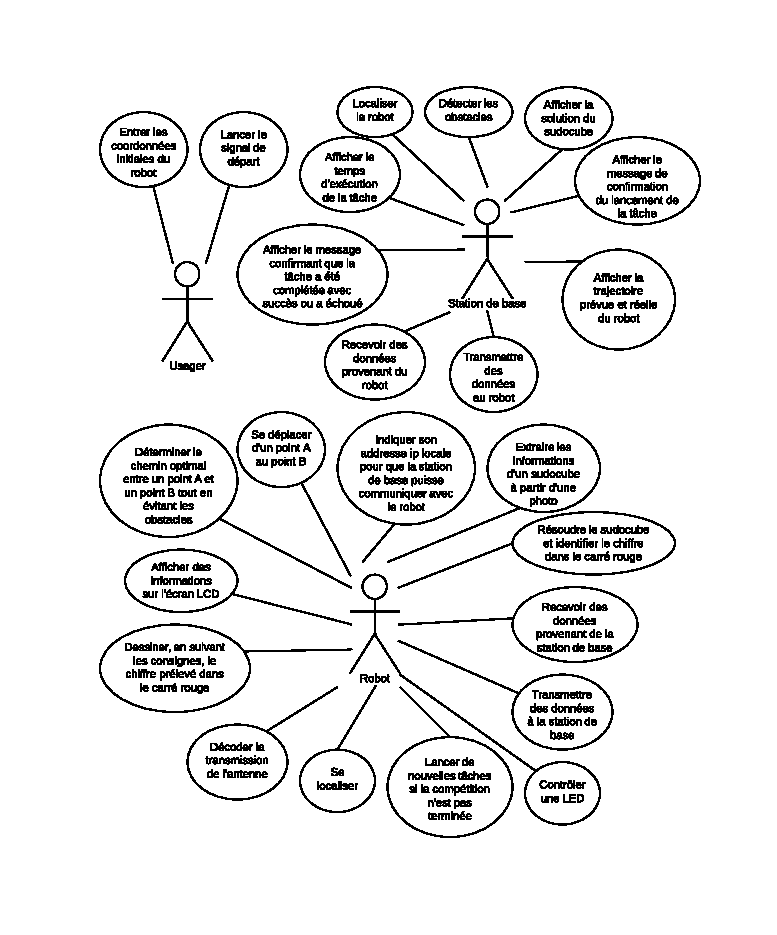
\includepdf[scale= 1]{use_cases_diagram.pdf}
%!TEX root = ../rapport.tex
%!TEX encoding = UTF-8 Unicode

% Chapitres "Introduction"

% modifié par Francis Valois, Université Laval
% 31/01/2011 - version 1.0 - Création du document

\chapter{Diagrammes de séquences}
\label{s:sequences}

%!TEX root = ../rapport.tex
%!TEX encoding = UTF-8 Unicode

% Chapitres "Introduction"

% modifié par Francis Valois, Université Laval
% 31/01/2011 - version 1.0 - Création du document
\chapter{Diagrammes de classes}
	\label{s:classes}
	\addtolength{\evensidemargin}{-1in}	

\begin{figure}[htbp]
\centering
\label{fig:DiagrammeClasse}
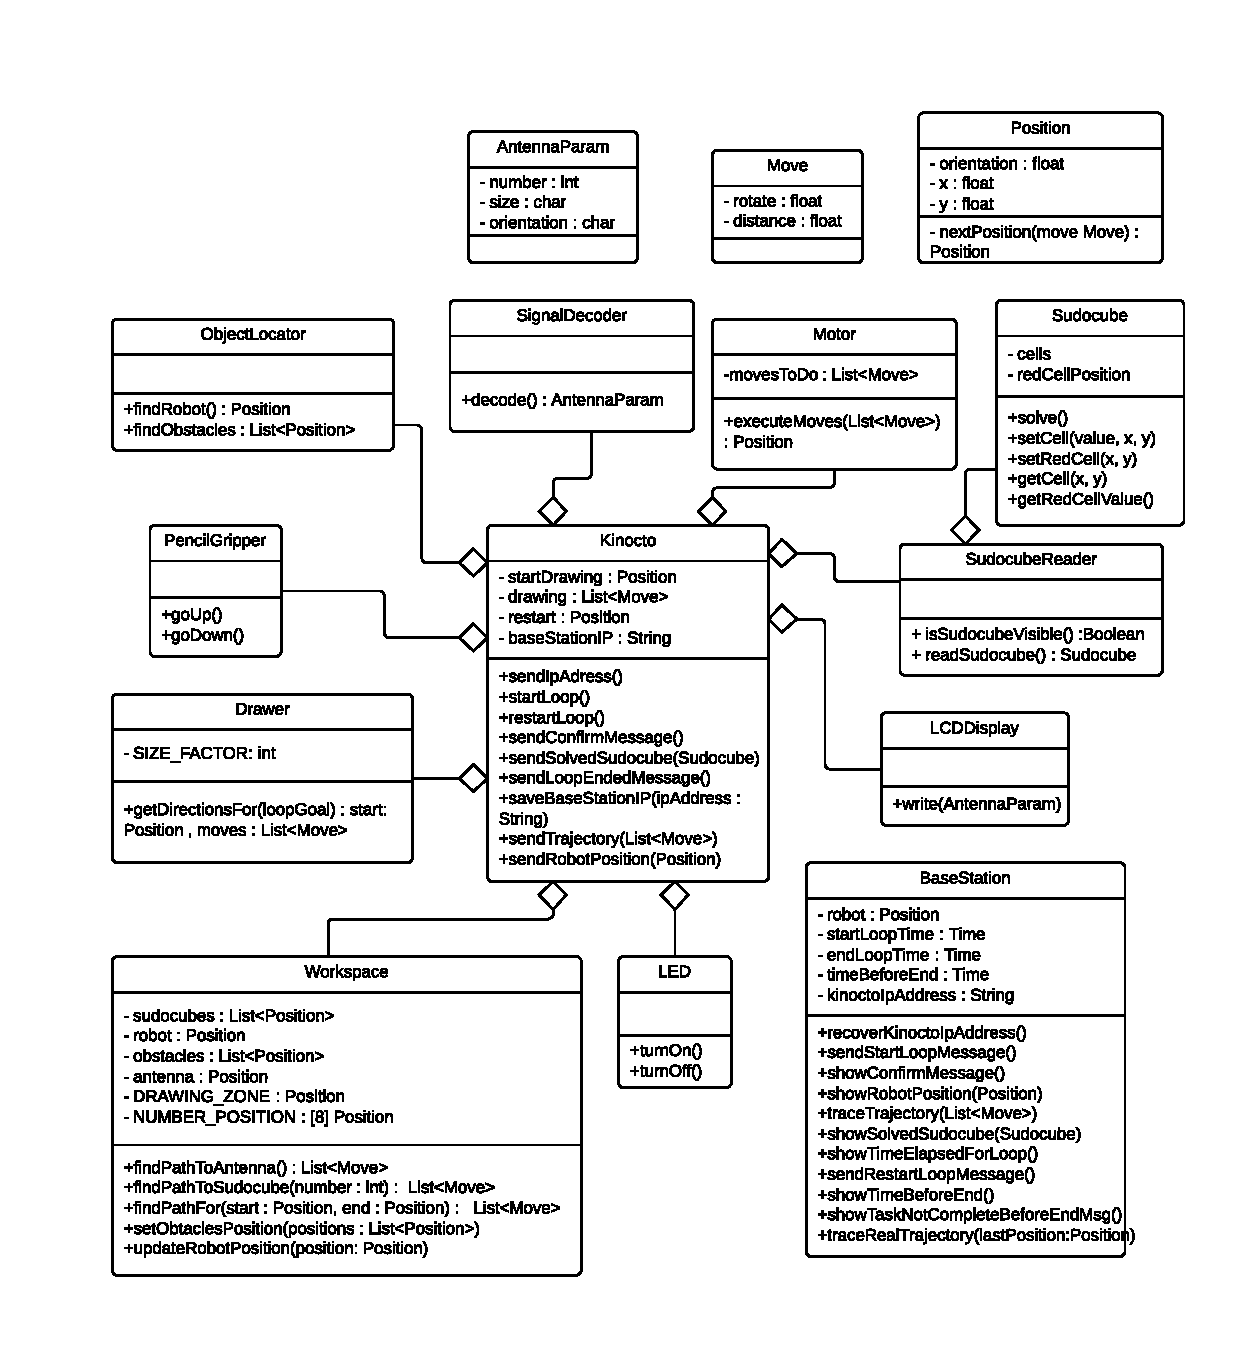
\includegraphics[scale=0.60]{fig/class_diagram.pdf}
\caption{Figure présentant le diagramme de classes du projet}
\end{figure}

%!TEX root = ../rapport.tex
%!TEX encoding = UTF-8 Unicode

% Chapitres "Introduction"

% modifié par Francis Valois, Université Laval
% 31/01/2011 - version 1.0 - Création du document

\chapter{Description des prototypes}
\label{s:prototypes}
\section{Préhenseur}

Comme dispositif pour le traçage des dessins par le robot, nous opterons pour une solution simple et robuste. Afin d’éviter d’augmenter inutilement la charge de travail du microcontrôleur, nous avons décidé d’éviter d’utiliser des solutions complexes qui pourraient exiger la production d’un signal particulier par le microcontrôleur. Le signal de sortie qui devra être produit sera simplement un signal binaire : « 1» lorsque le crayon devra être en mode traçage et « 0 » lorsque le crayon sera soulevé et donc en mode « attente ». Pour maintenir le crayon en position « attente » durant la durée du trajet, nous utiliserons un système de maintien magnétique qui gardera le crayon en position relevé lorsqu’il recevra le signal « 1 » logique. Pour abaisser le crayon et ainsi entrer en mode traçage, nous utiliserons un ressort à faible constante de rappel qui entrera en jeu lorsque le système de maintien magnétique relâchera le crayon « 0 » logique. Il est bien important que la constante de rappel du ressort soit faible pour ne pas briser la mine lors du contact de celle-ci avec la surface de traçage. La constante de rappel du ressort devra également être inférieure à la force exercée par le système de maintien magnétique qui relèvera le crayon en mode attente, une fois le dessin terminé.

\section{Récepteur et décodeur du signal Manchester}

Pour le récepteur du signal magnétique, nous utiliserons un « tone decoder » qui est utilisé dans de nombreuses applications qui nécessitent la reconnaissance de certaines tonalités bien précises. Comme nous avons besoin de détecter une série de tonalités identiques qui se suivent en formant un code, ce genre de dispositif nous convient parfaitement. Le « tone decoder » recevra le signal par une boucle de fil installée à un endroit sur le robot qui captera la variation du flux magnétique produite par le fil sous la table et détectera si la tonalité inaudible est émise ou non. Lorsque la fréquence (ou tonalité) sera reçue par le récepteur, celui-ci présentera zéro volt en sortie et à l’opposé, lorsque le récepteur ne détectera pas la fréquence ciblée, il présentera 5V à sa sortie. Il exécutera ces opérations d’une façon suffisamment rapide pour que le segment binaire reçu soit exactement le même que celui transmis, mais complètement opposé étant donné la configuration logique du « tone decoder ».  Ce message sera ensuite inversé par l’unité de traitement suivante et traité pour que le robot exécute la tâche adéquate. L’avantage de cette approche est que le « tone decoder » est un circuit intégré très robuste aux perturbations magnétiques de son environnement, il est peu énergivore et très compact.

\section{Microcontrôleur} \label{s:micro}

La composante qui effectuera le lien entre le pont en H qui contrôle les moteurs, les encodeurs sur les moteurs, le signal décodé par le récepteur du signal d'antenne, le préhenseur, la D.E.L., l'écran LCD et le Mac mini sera un microcontrôleur modèle Texas Instrument Stellaris LM3S9B92. Nous avons choisi ce microcontrôleur, car il possède un grand nombre de broches d'entrée/sortie, 4 sorties de signaux PWM, 2 interfaces d'encodeur à quadrature qui permettront le contrôle et l'asservissement des moteurs et il possède également deux ports de communication UART ainsi qu'une interface USB pour la communication avec le Mac mini. De plus, le microcontrôleur est programmé en C à l'aide d'un compilateur, d'un IDE et de librairies de pilotes de périphériques fournies.   

\section{Affichage sur le robot} \label{s:LCD}

Pour afficher les informations nécessaires sur le robot, nous utiliserons un écran à cristaux liquides 16 x 2  caractères. Cet écran est commandé par 8 lignes de données qui permettent de transmettre des caractères ASCII et 3 lignes de contrôle, RS, R/W et E. Le huitième bit de données peut également servir de « busy flag », ce qui permet de savoir si le contrôleur de l'écran a terminé d'exécuter les dernières instructions. En plus de la banque de caractères prédéfinie, il est possible d'ajouter des caractères "maison" dans des espaces libres de la mémoire de caractères. Le contraste peut être contrôlé par un potentiomètre qui fournit la référence sur la broche 3. En ce qui concerne l'alimentation, l'écran peut être alimenté à partir du microcontrôleur, en excluant le rétroéclairage, qui n'est pas nécessaire pour distinguer les caractères dans un environnement éclairé. Si le rétroéclairage devait être utilisé, il serait nécessaire de l'alimenter à l'aide d'une source indépendante du microcontrôleur, car il nécessite 150 mA. Les fonctions codées dans les fichiers ecran.h et ecran.c de l'annexe \ref{s:code_LCD} permettent d'envoyer des caractères et des chaînes de caractères sur le LCD et de contrôler le déplacement du curseur.

\section{Communication entre le microcontrôleur et le Mac mini} \label{s:comm_mac_micro}

Comme le microcontrôleur possède une interface USB qui permet la communication avec l'ordinateur par un port série UART, nous utiliserons ce protocole pour communiquer. Le port UART lève une interruption lorsqu'il reçoit un caractère dans son registre de données. Les données reçues peuvent être enregistrées dans un tampon circulaire durant l'interruption pour être traitées dans le processus principal. Du côté du Mac mini, un terminal série permettra d'envoyer des données par l'interface USB. 

\section{Alimentation du Mac mini} \label{s:alim_mac_mini}
En ce qui a trait au système d'alimentation du Mac mini, le dispositif à concevoir doit réussir à élever la tension de la pile jusqu'à 24V. Cette tension correspond à un point de fonctionnement qui est jugé comme idéal selon les spécifications techniques de l'appareil. On constate par la suite que la puissance demandée par le Mac mini sera la plus grande dépense énergétique du système. Il faut donc envisager une alimentation avec un très bon rendement, de manière à limiter le dimensionnement de la pile. L'usage d'un régulateur de tension conventionnel, qui utilise une tension supérieure à l'alimentation, n'est pas envisageable pour le projet, dans la mesure où le rendement dépasse rarement les 50\%. Ce qui s'offre à la conception de l'alimentation est un système de type «Boost» qui effectue une amplification de la tension continue. Ce type de circuit est le pendant en tension continue du transformateur. En soi, il est possible de réaliser la fonction d'amplification au moyen de composants discrets. Cependant, l'implantation pratique demande beaucoup de temps et de ressources et est généralement moins robuste qu'une alimentation utilisant des composants intégrés. Il est préférable, vu les coûts de l'électronique actuelle, d'opter pour des composants intégrés qui effectuent le même travail avec des rendements très élevés (de l'ordre du 90\% et plus). Aussi, vu le coût de l'ordinateur et sa sensibilité aux oscillations de tension, il est très important de considérer la stabilité de la tension de sortie de l'alimentation. Les régulateurs envisageables pour l'application et les spécifications en courant présentent une ondulation de tension inférieure aux niveaux maximaux du Mac mini ($\pm 200mV$). Il est donc tout indiqué d'opter pour un circuit intégré de type «Boost», vu son bon rendement, sa robustesse, sa facilité d'implantation ainsi que sa stabilité de tension de sortie.

\section{Alimentation de l'électronique embarquée}
En ce qui a trait au système d'alimentation de l'électronique embarquée, l'alimentation de l'électronique autre que le Mac mini doit se faire optimalement en 5V, puisqu'il s'agit d'une tension utilisable pour le servomoteur de la tourelle de la caméra et permet aussi de donner un point de référence au pont en H. Par ailleurs, la plupart des microcontrôleurs ont des entrées 5V, il est donc de mise d'utiliser cette tension pour l'électronique auxiliaire. Le dispositif devra abaisser la tension de la pile à 5V puisque celle-ci sera sélectionnée avec une tension supérieure. On peut tout de suite penser à l'usage d'un régulateur, cependant, pour les mêmes raisons qu'énoncées à la section \ref{s:alim_mac_mini}, un faible rendement de l'alimentation pourrait dégrader la durée de vie de la pile. Vu qu'il est nécessaire d'abaisser la tension, l'utilisation d'une technologie de type «Boost» est impossible. Il existe cependant la technologie de type «Buck», qui produit exactement l'effet contraire. L'utilisation de composés discrets requiert davantage de temps et est moins robuste. Une solution impliquant des composés intégrés doit être envisagée. Par ailleurs, les rendements de ce type d'alimentation peuvent s'élever à plus de 90\%. Les composantes comme le microcontrôleur et le pont en H requièrent une tension d'alimentation stable et l'emploi d'une alimentation faite à partir de composants intégrés permet de convenir à ce besoin. Il est donc tout indiqué d'opter pour un circuit intégré de type «Buck», vu son bon rendement, sa robustesse, sa facilité d'implantation ainsi que sa stabilité de tension de sortie.

\section{Communication sans fil}\label{s:sansfil}
Pour amorcer la communication sans fil entre le robot et la station de base, il faut que cette dernière sache l'adresse IP du robot. Il nous est impossible de brancher un clavier et un écran sur le robot afin de récupérer celle-ci et le réseau sans fil de l'université empêche l'utilisation de service tel que www.NOIP.com pour obtenir de façon dynamique l'IP de la carte réseau. Nous avons donc créé un script «bash» pour récupérer l'adresse IP du robot et l'envoyer à une application en ligne appelée «Pastebin» qui permet d'enregistrer du texte. Le script est placé dans le fichier «/etc/rc.d/rc.local» afin qu'à chaque démarrage, l'adresse IP soit connue. Pour valider l'adresse IP obtenue, il suffit d'essayer de se connecter par «SSH» sur le robot ce qui confirme la possibilité d'utiliser le réseau sans fil pour communiquer avec le robot.

Ultérieurement, nous utiliserons une api en C++ ou en Python pour communiquer.

\section{Lecture des informations d'un sudocube avec la caméra}
Pour réaliser ce prototype, OpenCV fut utilisé ainsi que quelques photos des sudocubes de l’environnement de travail du robot. Le langage de programmation C++ fut employé afin de garantir un temps de traitement relativement faible. Les opérations sur les images exigeant beaucoup de cycles processeur. De plus, l'accès à un plus grand nombre d'exemples de code OpenCV en C++(contrairement au Python) a aussi motivé le choix de ce langage.

L'algorithme testé dans ce prototype commence par effectuer une segmentation par couleur verte sur la photo afin d'isoler le cadre du sudocube. Puis, un algorithme de détection des contours est appliqué. OpenCV retourne, après ces opérations, deux polygones rectangulaires que l'on peut utiliser pour vérifier l'existence du cadre vert dans l'image. On s'assure que le cadre remplit une bonne partie de l'image en calculant l'aire de celui-ci. Cela permet de garantir qu'il y a assez de détails pour lire correctement les cases du sudocube. Ensuite, l'image originale est convertie en tons de gris pour appliquer encore une fois un algorithme de détection des contours. Cela permet de récupérer les polygones de toutes les cases du sudocube. Comme il y a quelques polygones qui ne sont pas des cases, on les élimine en calculant leur aire et en ne gardant que ceux qui sont suffisamment grands.

Afin de garantir la lecture de toutes les cases du sudocube, on pourrait ajouter une détection automatique du seuil de l'algorithme de détection des contours en vérifiant le nombre de polygones trouvés. Il faut en trouver exactement 47.

De plus, pour assurer une bonne lecture des caractères, on pourrait effectuer un réalignement du cadre vert.

Ce qui reste à faire : effectuer une segmentation sur la couleur rouge en mode HSV afin d'identifier la case rouge et créer un algorithme de reconnaissance des caractères pour lire les chiffres dans les cases.

\section{Recherche de chemin}
Afin de résoudre le problème de recherche d'un chemin à parcourir par le robot Kinocto afin d'éviter les obstacles, nous avons dû nous pencher sur certaines contraintes particulières à notre situation. Nous avons tout d'abord décidé de représenter la table à l'aide d'un nuage de points quadrillés, un peu à la manière d'un graphe ayant des coordonnées (x,y). Ce type de représentation facilite beaucoup la recherche de chemin puisque les algorithmes les plus efficaces travaillent sur des graphes. Par la suite, il a fallu considérer que notre robot n'est pas un point ponctuel sur la table. Ce problème a été contourné en insérant une marge autour des obstacles. En ayant des obstacles plus gros, ceci nous permet de garder une représentation du robot comme un point et utiliser un algorithme de recherche de chemin. L'algorithme A* a été choisi, car il est très rapide et facile à implémenter. Finalement, il y a une dernière contrainte à considérer, venant du fait que nous utilisons un nuage de point comme référence sur la table. Il est impossible de se déplacer en diagonale sans "zigzaguer" à travers les obstacles. Ceci engendre beaucoup de rotations nécessaires afin d'arriver au point final ce qui contribue à l'incertitude de la position réelle du robot. Nous ajouterons donc une couche logicielle permettant d'identifier les points critiques du chemin trouvé par l'algorithme A*. Ainsi, cette liste de points permettra au robot de se déplacer en ligne droite lorsqu'il fera des diagonales en ignorant les points inutiles entre les points critiques qui créaient le mouvement involontaire, et réduira par le fait même le nombre de rotations nécessaires avant d'arriver au point final. 

\section{Kinect}
La Kinect est l’outil qui va nous aider à localiser les obstacles et localiser notre robot sur la table. Après l’installation d’OpenNI et OpenCV, nous avons testé la Kinect avec le fichier test.cpp qui permet de faire une capture d’image.\\
Pour localiser le robot par rapport à la Kinect, nous allons le modéliser avec une figure spécifique sur celui-ci (exemple : deux cercles). Ensuite, grâce à la connaissance de la distance entre les deux cercles, nous pourrons déterminer à chaque rafraichissement de position: la distance du robot par rapport à la kinect et par rapport aux obstacles ainsi que sa position angulaire approximative. Pour les équations, nous allons utiliser des équations simples comme les règles de trigonométrie. De plus, afin d'éviter le bruit dans nos images, il est judicieux d'appliquer des filtres correctifs. Le filtre passe-bas est le plus réputé pour enlever le bruit. Toutefois, il rend les images "flou", alors il faut chercher les meilleurs paramètres pour obtenir un filtre optimal et efficace. En ce qui concerne la détection d’obstacles, nous avons deux choix. Le premier choix consiste à faire une capture avec la caméra et en faire l’analyse 2D tandis que le deuxième choix consiste à utiliser l’image de profondeur. Pour le moment, la solution qui semble la plus efficace est l’utilisation de l’image de profondeur qui consiste tout d'abord à isoler l'obstacle qui possède une forme déjà connue et conserver les points dont la profondeur est proche de celle des obstacles. Par la suite, nous conservons une image en teinte de gris, car c'est le contour de l'obstacle qui nous intéresse. Finalement, on se sert d'OpenCV pour définir un détourage de l'obstacle et l'affiner. 


\appendix
%!TEX root = ../rapport.tex
%!TEX encoding = UTF-8 Unicode
% Chapitres "Annexes"

% modifié par Francis Valois, Université Laval
% 31/01/2011 - version 1.0 - Création du document
\chapter{Annexes}
\label{s:annexes}

\section{Asservissement des moteurs}
\subsection{Fonction agissant comme PID} \label{s:fonction_PID}
\begin{lstlisting}[language=C]
long PIDHandler(volatile long *consigne, volatile long *measured_value, volatile float *I, volatile long *previous_error, float dt)
{
  long error = *consigne - *measured_value;
  *I = *I + error*dt;
  float D = (error - *previous_error)/dt;
  long output = Kp*error + Ki*(*I) + Kd*D;
  *previous_error = error;
  return output;
}
\end{lstlisting}



\end{document}
% Fin du document

